\vspace{1.0cm}
\section{Description of the Markets and Data}
\subsection{Industrial Characteristics}
\subsubsection{Taxi Market}
\hspace{0.5cm} In NYC, yellow cabs are regulated by NYC Taxi and Limousine Commission (TLC). Each taxicab vehicle has to be equipped with a medallion, a small metal plate and license required to operate taxicabs in NYC and issued by TLC.\footnote{The word "(yellow) medallion" is often used to mean just yellow cabs. I follow this convention in this paper and use the both words interchangeably.} The authority controls the fare system, the (maximum) number of medallions and so on.\footnote{See the classic paper, Schreider (1975 \cite{shreiber1975economic}) for theoretical reasons of those regulations.}  Street hail livery vehicles (as known as "boro taxis" or "green cabs") are another type of taxis also regulated by TLC. They have fare structure in common, but are different in that while yellow cabs can pick passengers up at any spot in 5 boroughs in NYC (Manhattan, Brooklyn, the Bronx, Queens, and Staten Island), boro taxis are prohibited to pick them up at Manhattan (excluding the northern districts) and the airports, John F. Kennedy and LaGuardia.\footnote{As boro taxis are the livery services, passengers can call the base for pre-arranged trips and also negotiate prices in that case. Only for pre-arranged trips can passengers get on boro taxis from airports.} See the map in Figure \ref{fig:map_service_area}.

The taxi market in NYC is large. According to Buchholz (2016), approximately 700 million passengers get on taxis in 2013 in the United States and NYC consists of as much as 34\% of the number. In revenues, NYC generates about 4 billion dollars annually, which is 25 \% of the whole U.S. market.

There are mainly two types of medallions. One is corporate medallion, so-called "minifleet", owned by corporations and can be leased out to individual drivers or the companies can hire employees to drive. They were requested to drive two shifts per day including weekends and holidays, and each shift had to be longer than 9 hours. The restriction was removed in February 2015 for the sake of more flexibility.\footnote{http://www.nyc.gov/html/tlc/downloads/pdf/newly\_passed\_rule\_drv\_veh\_owner\_updated.pdf} The other type is owner-owned medallion. Some individual drivers own and drive medallions and can decide when and how much to work flexibly. There was once a regulation, known as owner-must-drive, that they had to drive at least 210 nine-hour shifts a year and if they violated, they had to pay fines. This restriction was also removed in February 2016.\footnote{http://www.nyc.gov/html/tlc/downloads/pdf/proposed\_rules\_omd\_repeal\_2016.pdf} These restrictions partially justify fixing the number of medallions conditional on locations and dates in my model. According to 2014 TLC Factbook, approximately 60\% of medallions are minifleets and the rest is owner-operated ones and the Factbook (2016 version) shows that there are 13,587 yellow cabs (and 7,676 boro taxis) in NYC.\footnote{These numbers, combined with evidence from Frechette et al.(2016), are used later to calculate the number of medallions in my model.} Medallions can be traded in the market. They were once sold for more than 1.3 million dollars in 2013 but plummeted to just 241,000 dollars in 2017, and the main reason would be the rise of ride-hailing services.\footnote{http://nypost.com/2017/04/05/taxi-medallions-reach-lowest-value-of-21st-century/}

\begin{figure}[h]
\centering
\caption{Map of Service Area}\label{fig:map_service_area}\\
\vspace{0.2cm}
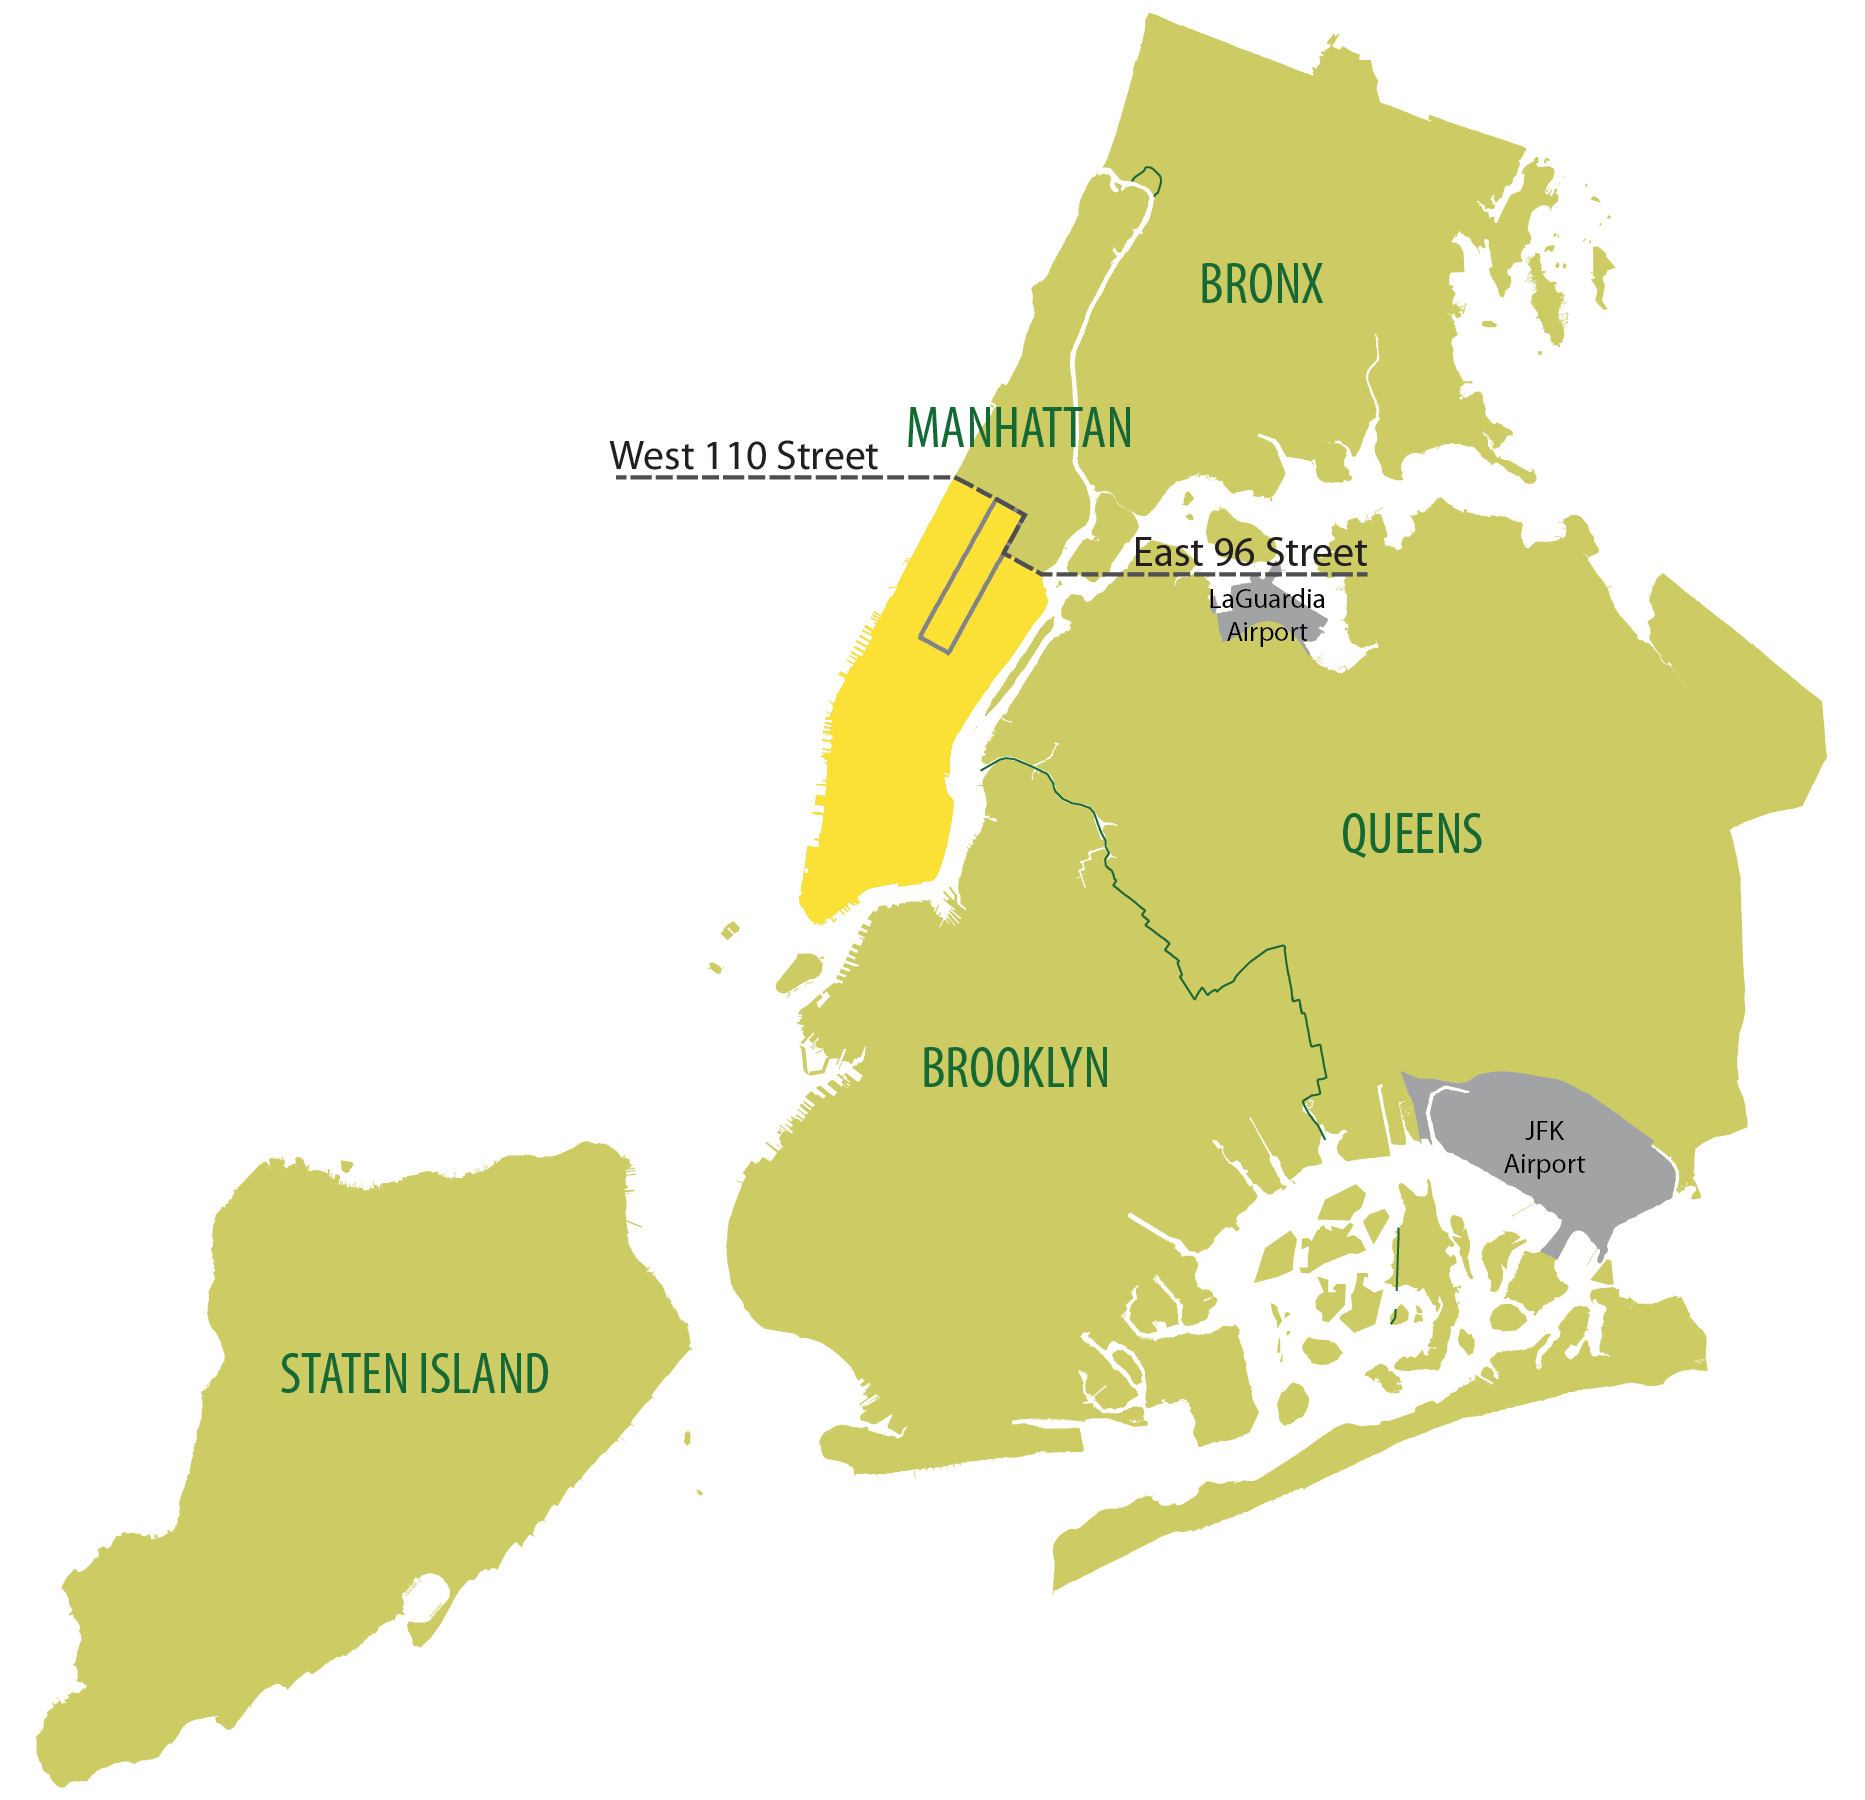
\includegraphics[width=12cm]{Figures/map_service_area.png}
{\footnotesize \noindent Source: TLC}
\end{figure}


\vspace{0.5cm}
\subsubsection{Ride-Hailing Market}
\hspace{0.5cm} Ride-hailing services have become popular dramatically in 2010's, taking advantage of the development of information technology and the emergence of smartphones.\footnote{Ride-hailing markets, sometimes called ride-sharing markets, are considered as an industry of sharing economy or "gig" economy, whose essence is that there are underutilized goods (cars) owned by some individuals, and both owners and non-owners benefit from consuming those goods together via transferring rents. The ride-hailing service is unique in that car owners also provide their labors.} They were successful in mitigating the inefficiencies of taxis such as search frictions, illiquidity of prices and the fixed (maximum) number of vehicles. The market leader, Uber, has more than 70 \% shares (2016, based on the number of trips) in NYC and operates globally, and it became so popular that the word "Uber" is now used as a verb or the phenomenon is referred to "Uberfication".\footnote{There is still plenty of room to expand dramatically. Lashinsky (2017 \cite{wildride2017}) discloses that though about half of Americans have ever heard of ride-hailing, just 15\% have an experience of the service.} Cars used in the service are mainly privately owned by drivers and not for the commercial purpose originally. Drivers are also very flexible about when and how much to supply their labors. Candidate drivers in NYC attend 24-hour FHV class at TLC-approved school and take a defensive driving course to be drivers. The number of active drivers is growing rapidly and the number of weekly vehicles dispatched by Uber surpassed the number of yellow cabs in May 2015, and even Lyft, the second biggest U.S. ride-hailing service which has approximately 10\% market share (2016) in NYC, also dispatched more vehicles than yellow cabs.\footnote{http://toddwschneider.com/posts/taxi-uber-lyft-usage-new-york-city/} Note that while most taxi drivers work full time, drivers serving for ride-hailing markets are often part-timers, and many drivers work for both Uber and Lyft, so the number of dispatched vehicle somewhat overestimates the capacity of supply by ride-hailing services.

Those companies provide various types of ride-hailing services in NYC. I take Uber for example. The closest substitute to taxis is UberX, which is launched in September 2011 in NYC, driven by standard sedan and most popular\footnote{There are also services by van for higher capacity called UberXL whose fare is slightly higher.}. As written later, Uber cut its fare in January 2016 and became cheaper than taxis on average. According to Cohen et al. (2016), UberX represents approximately 80\% of all service by Uber, and thus when I refer to Uber or ride-hailing services in this paper, UberX or its equivalent is in mind. Some premium car services like UberBlack are also provided. There is also a service of sharing of ride-sharing, UberPOOL, where passengers who head for the same direction with near pickup/dropoff locations are matched. It started from January 2015 in NYC, with lower fare than UberX. Uber has an algorithm to increase the price when demand is high, so-called "surge pricing" whose detail is not disclosed.\footnote{Chen et al. (2015 \cite{chen2015peeking}) partially disclose how it works by creating dummy accounts and using public Uber API, and show their concerns about its fairness and transparency.} The algorithm makes it possible to efficiently dispatch cars to waiting passengers and to raise fare when the market is tight so that only passengers with high valuation request cars and drivers are incentivized.\footnote{Cramer and Kruger (2016 \cite{cramer2016disruptive}) compare the efficiency of taxis with that of ride-hailing services with respect to capacity utilization rate in five cities in the U.S. and conclude that it is much higher for Uber drivers than taxi drivers in most cities. Interestingly, the only exception is NYC, where the utilization rate is almost identical between taxis and Uber. This would be because highly densely populated NYC makes efficient matching possible.} Lyft and other ride-hailing companies also provide similar services, though some don't apply price alternation mechanism. 



\vspace{0.5cm}
\subsection{Data and Descriptive Evidence}
\subsubsection{Data}
\hspace{0.5cm} Data I use in this paper are mainly based on Taxicab \& Livery Passenger Enhancement Programs (TPEP/LPEP) data disclosed by TLC, which include all individual trips by yellow cabs since 2009, boro taxis (green cabs) since its launch in August 2013, and For-Hire Vehicle (FHV) including Uber and Lyft since 2015.\footnote{http://www.nyc.gov/html/tlc/html/about/trip\_record\_data.shtml} For yellow cabs and boro taxis, each trip data has pickup and dropoff time, trip distance, pickup/dropoff longitude and latitude\footnote{Since July 2016, these are replaced by location ID in the same way as FHV.}, pricing scheme (standard, John F. Kennedy Airport, etc.), payment method (cash or card), fare amounts, surcharges/tolls, tips amount (only when paid by credit card) and so on. Unfortunately, there is no data who the drivers were or which cabs were used for each trip (such as hack number or medallion IDs), so I don’t know each driver’s supply, let alone when and how long they were searching for potential passengers. With respect to FHV, the available data are limited and only contain dispatcher ID (no driver identified, but able to distinguish Uber from other Limo services, for example), pickup time and location ID showing rough location almost the same as in Figure \ref{fig:Manhattan} in the next section. 

\subsubsection{Summary of TLC Data}
\hspace{0.5cm} The number of average daily trips in the whole New York City from 2013 to 2016 is summarized in Figure \ref{fig:Daily_trips}. Though not shown in the figure, trips by yellow cabs from 2009 and 2012 are very similar with those of 2013. Limo and Black car services are excluded. Since TLC doesn't have trip data of FHV before 2015, these numbers are just set to be 0. Though there were certainly some trips completed by ride-hailing services during the period, various evidence implies that the number is almost negligible compared to that by taxis.\footnote{For example, see http://toddwschneider.com/posts/analyzing-1-1-billion-nyc-taxi-and-uber-trips-with-a-vengeance/} As expected, the number of trips by yellow cabs have declined in these days, while the number of trips by ride-hailing companies has grown at a significant pace\footnote{This is the sum of the trips by Uber, Lyft, Via, Gett, and Juno.}, and the total demand for taxi-like transportation actually has increased from approximately 500,000 to 700,000.


\begin{figure}[h]
\centering
\caption{Daily Trips (2013-2016)}\label{fig:Daily_trips}\\
\vspace{0.2cm}
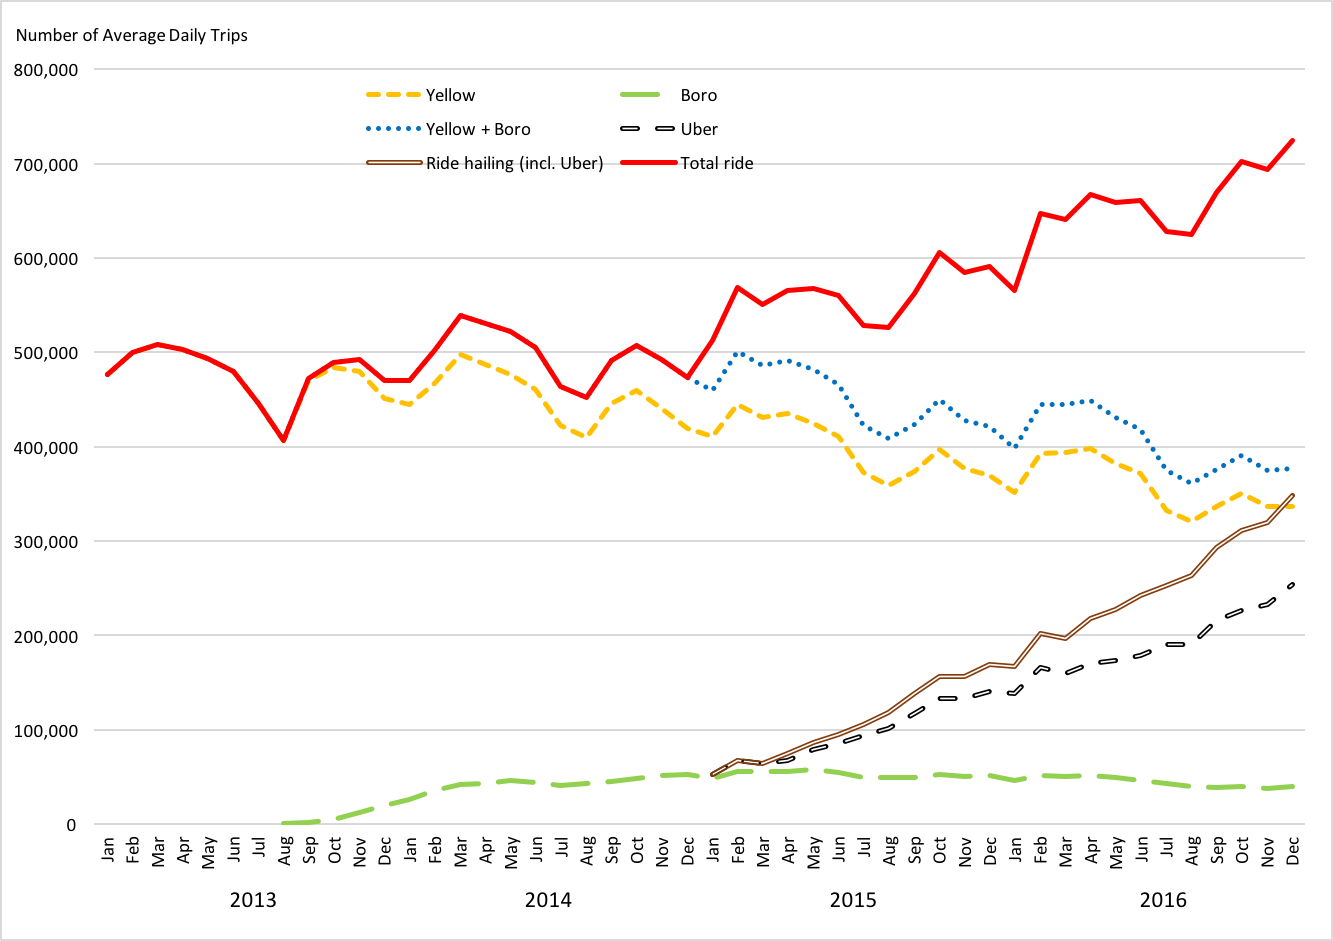
\includegraphics[width=12cm]{Figures/Daily_trips.png}
\end{figure}


\indent The following Figures \ref{fig:pickdrop_yellow} to \ref{fig:pickdrop_uber} show the distribution of trips which started/ended at each borough/district by yellow cabs, boro taxis, and Uber in July 2016. As TLC has no data of dropoff locations of trips by Uber, only distribution by pickup locations is in the chart. Other or unknown districts include New Jersey/ New Ark airport.\footnote{Passengers can get on yellow cabs only at New Ark airport in New Jersey. Yellow cab drivers are not authorized to pick passengers up on the road in New Jersey. http://frlimo0.tripod.com/njtaxiregulations.htm} 

\begin{figure}[h]
\centering
\caption{Distribution of Trips by Borough/District (Yellow Cabs)}\label{fig:pickdrop_yellow}\\
\vspace{0.2cm}
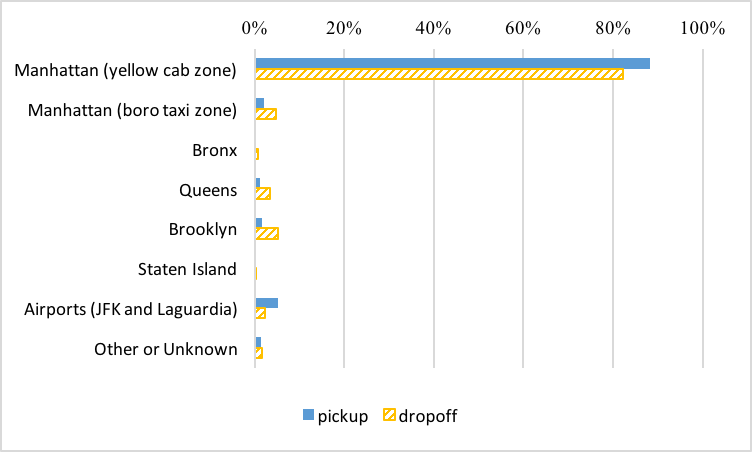
\includegraphics[width=8cm]{Figures/pickdrop_yellow.png}
\end{figure}

\begin{figure}[h]
\centering
\caption{Distribution of Trips by Borough/District (Boro Taxis)}\label{pickdrop_boro}\\
\vspace{0.2cm}
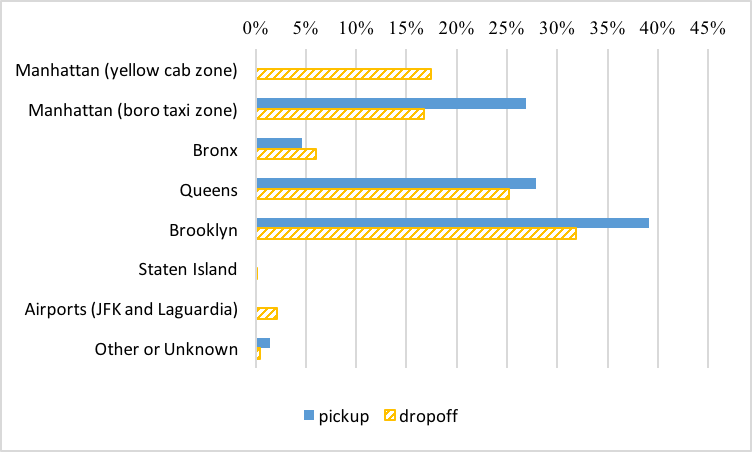
\includegraphics[width=8cm]{Figures/pickdrop_boro.png}
\end{figure}

\begin{figure}[h]
\centering
\caption{Distribution of Trips by Borough/District (Uber)}\label{fig:pickdrop_uber}\\
\vspace{0.2cm}
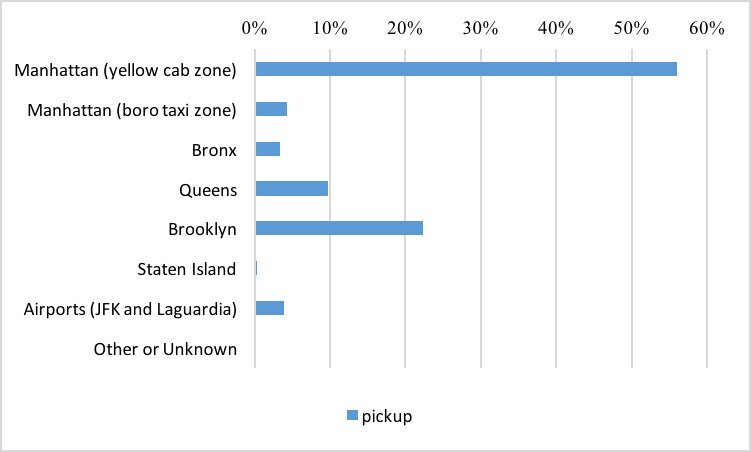
\includegraphics[width=8cm]{Figures/pickdrop_uber.png}
\end{figure}

As the figure indicates, more than 80 \% of trips by yellow cabs started or ended within yellow cab zones. Dropoff districts are relatively distributed. Regarding boro taxis, they can't be hailed within yellow cab zone in Manhattan and airports\footnote{There are some pickups by boro taxis at airports. This would be pre-arranged trips which are allowed as they are livery services.}, but they sometimes drop off in those areas. More than half of the trips started or ended outside Manhattan.

Though Uber drivers pick passengers up mainly in Manhattan, the percentage of pickups in outer boroughs, especially in Brooklyn, is higher than that by yellow cabs. This might be due to the situation that 1) passengers have to wait for yellow/green cabs for longer time in outer boroughs and thus Uber becomes more convenient and 2) they often take longer trips and therefore Uber is much cheaper than taxis.\footnote{See 3.2.4.}


\vspace{0.5cm}
\subsubsection{Taxi Fare Increase in September 2012}
\hspace{0.5cm} TLC raised the fare from 40 cents to 50 cents per 1/5 mile (or per 60 seconds when the traffic is slower than 12 mph) in September 2012. Base fare (first 1/5 mile) remained the same; 2.5 dollars.\footnote{This is standard fare system, which consists of most trips by yellow cabs. A typical exception is a trip between Manhattan and JFK airport. The rate is flat and rose from \$45 to \$52 by the fare increase.} Figure \ref{fig:Change_trips} shows how the number of trips in NYC changed before and after fare increase monthly, based on the different trips' distance. The horizontal axis is the distance in miles. Since the base fare was unchanged, the percentage of the fare increase is higher for longer trips. As the figure indicates, compared to the number of trips between September and July from 2011 to 2012, the equivalent number during the same period from 2012 to 2013 decreased by approximately 3.5\% on average, and this is not due to Uber.\footnote{I eliminated August because boro taxis were introduced in August 2013.} Actually, it is possible that supply increased (and hence expected wait time decreased) so that I underestimate the demand decrease.


\begin{figure}[h]
\centering
\caption{Change in the Number of Trips (2011-2012 vs 2012-2013)}\label{fig:Change_trips}\\
\vspace{0.2cm}
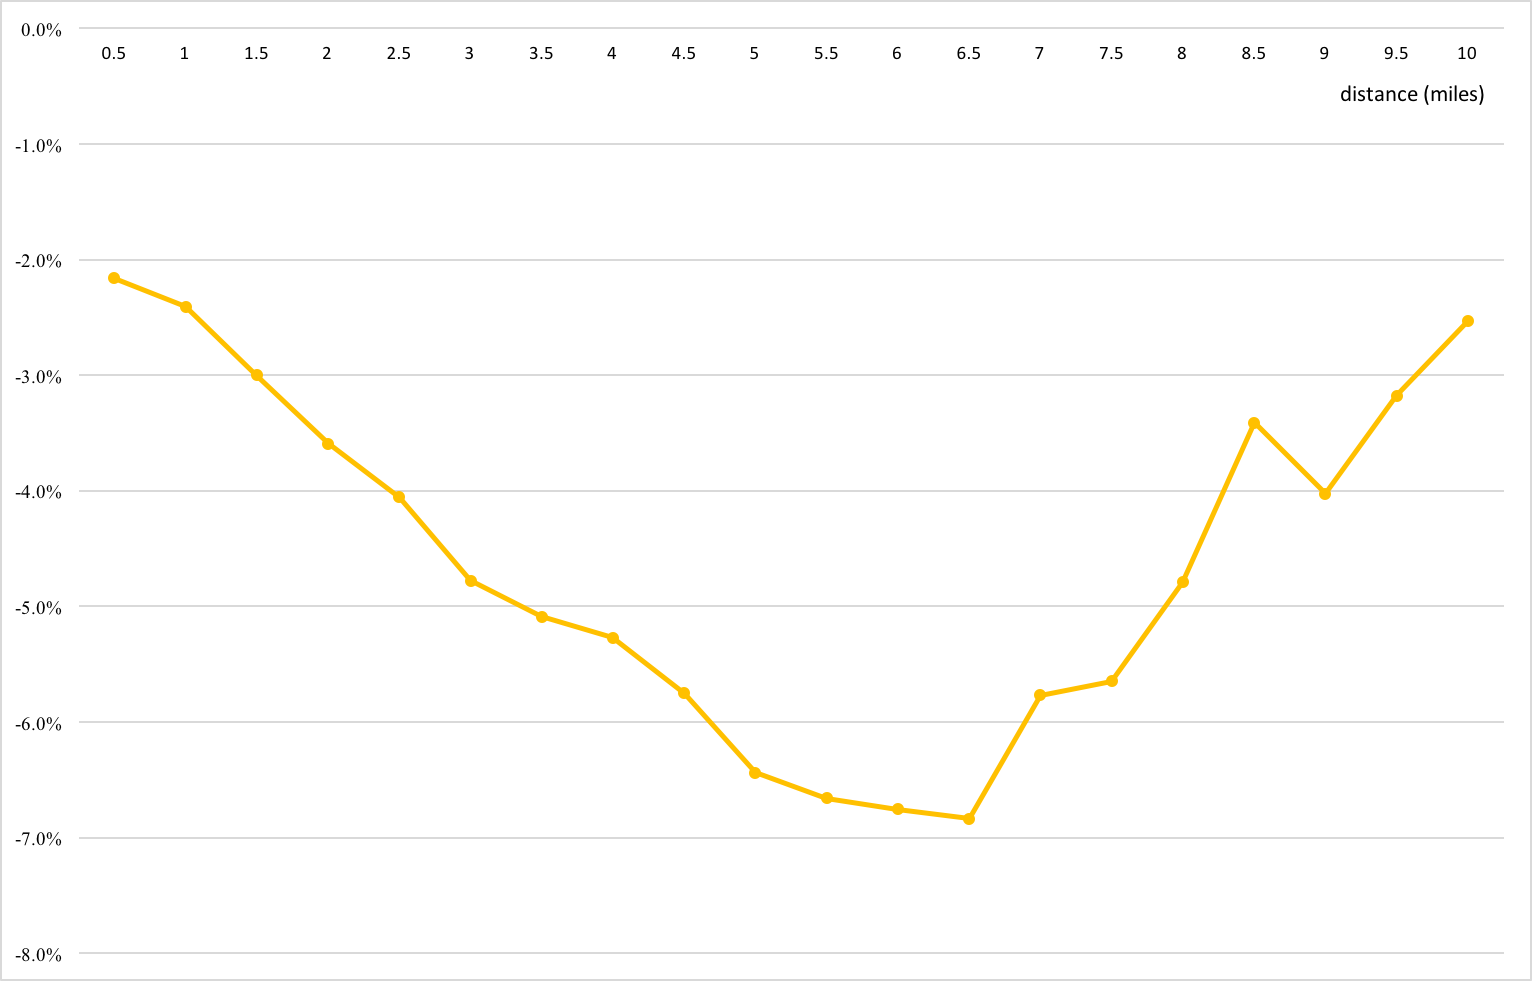
\includegraphics[width=12cm]{Figures/Change_trips.png}
\end{figure}

\\\indent As seen in Figure \ref{fig:Daily_trips}, the number of trips by yellow cabs started to significantly decline from 2014, but it would be natural to consider that the causes are mainly the introduction of boro taxis and rise of Uber. This might suggest that taxis and other public transportations are not so close substitute, while taxis and Uber are very close. I will see how demand changed by fare increase in the next section.


\vspace{0.5cm}
\subsubsection{Uber's Fare Cut}
\hspace{0.5cm} Uber cut its fare by approximately 15\% at the end of January 2016 and announced that the fare on average became lower than that of taxi's.\footnote{https://newsroom.uber.com/us-new-york/lower-prices-increased-demand/}. The following table\footnote{Fare on the table is that of UberX. I hereafter assume that all of the Uber trips were operated by UberX.} summarizes how fare changed before and after Uber's fare cut (and also yellow cab's fare increase). 

\begin{table}[h]
\begin{center}
\caption{Fare Comparison}\label{tab:fare_comparison}\\
\vspace{0.2cm}
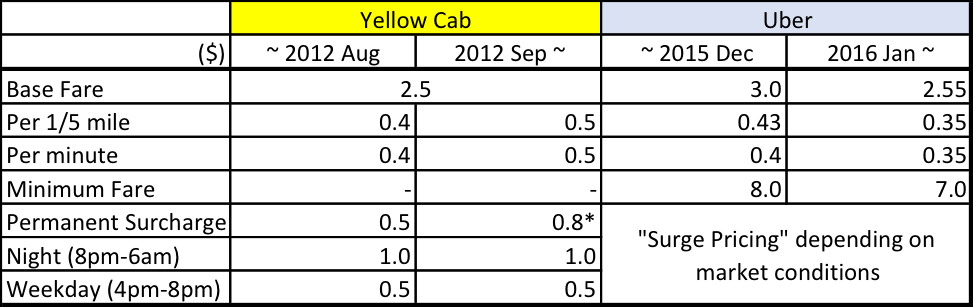
\includegraphics[width=12cm]{Tables/fare_comparison.png}
\end{center}
{\footnotesize \hspace{2.5cm} *Permanent surcharge rose to \$0.8 in January 2015.}
\end{table}

As at least \$0.8 surcharge is imposed on every taxi trip\footnote{For detailed information, see http://www.nyc.gov/html/tlc/html/passenger/taxicab\_rate.shtml}, base fare is virtually higher for taxis and per-1/5-mile fare\footnote{Uber discloses its fare system only per mile and it is not clear how many kinks there are within a mile. I just divide the per-mile-fare by 5.} is also higher for yellow cabs before and after Uber's fare cut, so whether Uber fare is higher or not depends on if the taxi fare is lower than Uber's minimum fare or not, except when the Uber's surge pricing is working.\footnote{Salnikov et al. (2015 \cite{salnikov2015openstreetcab}) study which one is cheaper using disclosed Uber API and develop a smartphone app to show their prices.} If tips are not considered, which is almost mandatory for yellow cabs but discouraged for Uber trips\footnote{Function of paying tips within smartphone app was not activated until 2017.}, the threshold in miles where Uber becomes cheaper is around 1.8 miles depending on days or time due to miscellaneous surcharges. In addition, whether fare of Uber trips actually decreased or not depends on distance; if it is longer than about 2.5 miles after fare cut, the fare actually decreased.\footnote{Time charge and surge pricing are not considered. See also Figure \ref{fig:elasticity_lnuber} in Section 5 for reference.} 
